\begin{enumerate}[label=\thesection.\arabic*.,ref=\thesection.\theenumi]
\numberwithin{equation}{enumi}
\item Lead compensator is used to reduce settlling time. Explain.\\
\\
\solution 
\\
\\
\textbf{unity feedback system}
\begin{figure}[h]
\begin{center}
\resizebox{\columnwidth}{!}{\tikzstyle{block} = [draw, fill=blue!20, rectangle, 
    minimum height=0.7cm, minimum width=0.7cm]
\tikzstyle{sum} = [draw, fill=blue!20, circle, node distance=1cm]
\tikzstyle{input} = [coordinate]
\tikzstyle{output} = [coordinate]
\tikzstyle{pinstyle} = [pin edge={to-,thin,black}]

\begin{tikzpicture}[auto, node distance=2.5cm,>=latex']
    % We start by placing the blocks
    \node [input, name=input] {};
    \node [sum, right of=input] (sum) {};
    \node [block, right of=sum] (controller) {H(s)};
    \node [output, right of=controller] (output) {};


    \draw [draw,->] (input) -- node {$R(s)\ +$} (sum);
    \draw [->] (sum) -- node {$E(s)$} (controller);
    \draw [->] (controller) -- node [name=y] {$Y(s)$}(output);
  \draw [->] (y) -- ++ (0,-2) -| node [pos=0.99] {$-$} (sum);
 
\end{tikzpicture}}
\end{center}
\end{figure}\\


 \textbf{compensated system}
\begin{figure}[h]
\begin{center}
\resizebox{\columnwidth}{!}{

\tikzstyle{block} = [draw, fill=blue!20, rectangle, 
    minimum height=3em, minimum width=6em]
\tikzstyle{sum} = [draw, fill=blue!20, circle, node distance=1cm]
\tikzstyle{input} = [coordinate]
\tikzstyle{output} = [coordinate]
\tikzstyle{pinstyle} = [pin edge={to-,thin,black}]

% The block diagram code is probably more verbose than necessary
\begin{tikzpicture}[auto, node distance=2cm,>=latex']
    % We start by placing the blocks
    \node [input, name=input] {};
    \node [sum, right of=input] (sum) {};
    \node [block, right of=sum] (controller) {G(s)};
    \node [block, right of=controller,
           node distance = 4cm ] (system) {D(s)};
    % We draw an edge between the controller and system block to 
    % calculate the coordinate u. We need it to place the measurement block. 
    \draw [->] (controller) -- node[name=u] {$U(s)$} (system);
    \node [output, right of=system] (output) {};
    \coordinate [below of=u] (tmp);

    % Once the nodes are placed, connecting them is easy. 
    \draw [draw,->] (input) -- node {$R(s)\ +$} (sum);
    \draw [->] (sum) -- node {} (controller);
    \draw [->] (system) -- node [name=y] {$Y(s)$}(output);
    \draw [->] (y) |- (tmp) -| node[pos=0.99] {$-$} 
        node [near end] {} (sum);
\end{tikzpicture}

}
\end{center}
\end{figure}\\
\textbf{Settling time - }\\
It is the time required for the response to reach the steady state and stay within the specified tolerance bands around the final value. In general, the tolerance bands are 2\% and 5\%.
\\
Lead compensator is used to reduce settling time - \\
\begin{align}
here, G(s) =  \frac{H(s)}{1+H(s)}
\end{align}
let,\\
\begin{align}
system-G(s) = \frac{1}{s(3s+1)}\\
lead\ compensator-D(s) = \frac{3(s+\frac{1}{3})}{(s+1)} \\
hence, new\ system-G_{1}(s) = \frac{1}{s(s+1)}
\end{align}
\\

\textbf{unit impulse response}\\
a). without lead compensator - \\
\begin{align}
G(s) = \frac{1}{(s)(3s+1)}\\
Y(s) = G(s).1\\
Y(s) = \frac{1}{(s)(3s+1)}
\end{align}
splitting into partial fractions\\
\begin{align}
Y(s) = \frac{1}{s} - \frac{1}{s+\frac{1}{3}}
\end{align}
taking inverse laplace transform, \\
\begin{align}
y(t) = [ 1 - e^{\frac{-t}{3}}]u(t)
\end{align}
\\
b). with lead compensator - \\
\begin{align}
G(s) = \frac{1}{(s)(3s+1)}\\
D(s) = \frac{3(s+\frac{1}{3})}{(s+1)} \\
G_{1}(s) = \frac{1}{s(s+1)}\\
Y_{1}(s) = G_{1}(s).1\\
Y_{1}(s) = \frac{1}{s(s+1)}
\end{align}
splitting into partial fractions\\
\begin{align}
Y_{1}(s) = \frac{1}{s} - \frac{1}{s+1}
\end{align}
taking inverse laplace transform, \\
\begin{align}
y(t) = [ 1 - e^{-t}]u(t)
\end{align}
\\
\textbf{unit step response}\\
a). without lead compensator - \\
\begin{align}
G(s) = \frac{1}{(s)(3s+1)}\\
Y(s) = G(s).\frac{1}{s}\\
Y(S) = \frac{1}{(s^2)(3s+1)}
\end{align}
splitting into partial fractions\\
\begin{align}
Y(s) = \frac{1}{s^2} + \frac{3}{s+\frac{1}{3}} + \frac{-3}{s}
\end{align}
taking inverse laplace transform, \\
\begin{align}
y(t) = [t + 3e^{\frac{-t}{3}} - 3]u(t)
\end{align}
\\
b). with lead compensator - \\
\begin{align}
G(s) = \frac{1}{(s)(3s+1)}\\
D(s) = \frac{3(s+\frac{1}{3})}{s+1} \\
G_{1}(s) = \frac{1}{s(s+1)}\\
Y_{1}(s) = G_{1}(s).\frac{1}{s}\\
Y_{1}(s) = \frac{1}{(s^2)(s+1)}
\end{align}
splitting into partial fractions\\
\begin{align}
Y_{1}(s) = \frac{1}{s^2} + \frac{1}{s+1} - \frac{1}{s}
\end{align}
taking inverse laplace transform, \\
\begin{align}
y(t) = [t + e^{-t} - 1]u(t)
\end{align}


\begin{figure}
\ \ \ \textbf{phase plot}\\
%\begin{subfigure}{\textwidth}
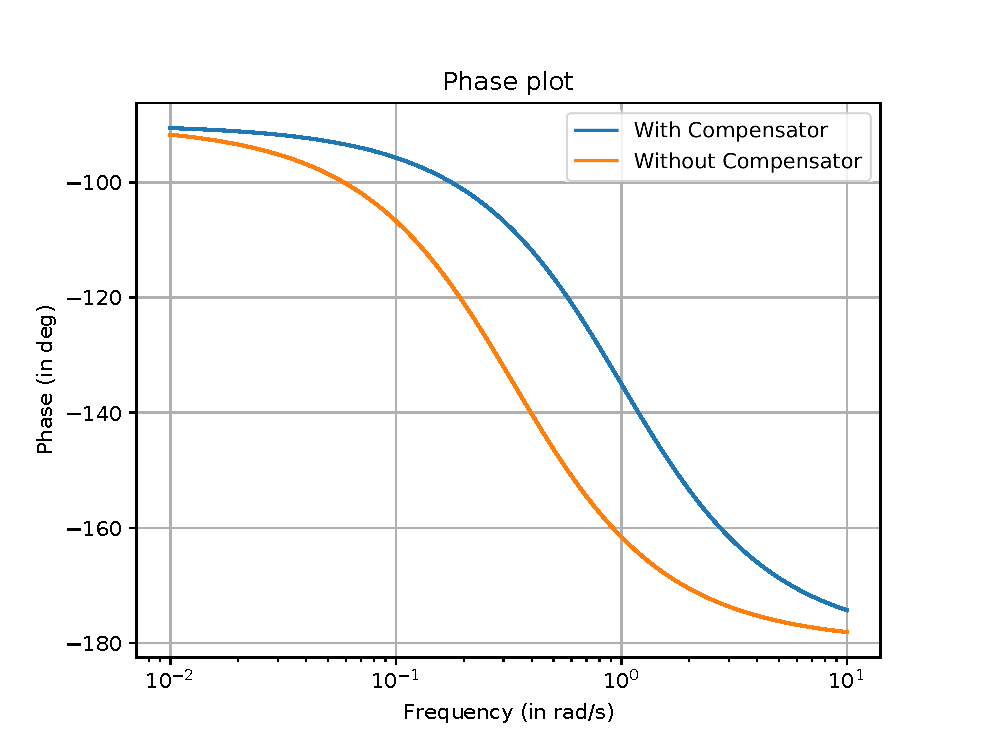
\includegraphics[width=1\linewidth, height=7cm ,inner]{./figs/ee18btech11027/lead_compensator_phase.eps} 
\label{fig:subim1}
%\end{subfigure}
\end{figure}

\begin{figure}
\ \ \ \textbf{reduced settling time}\\
%\begin{subfigure}{\textwidth}
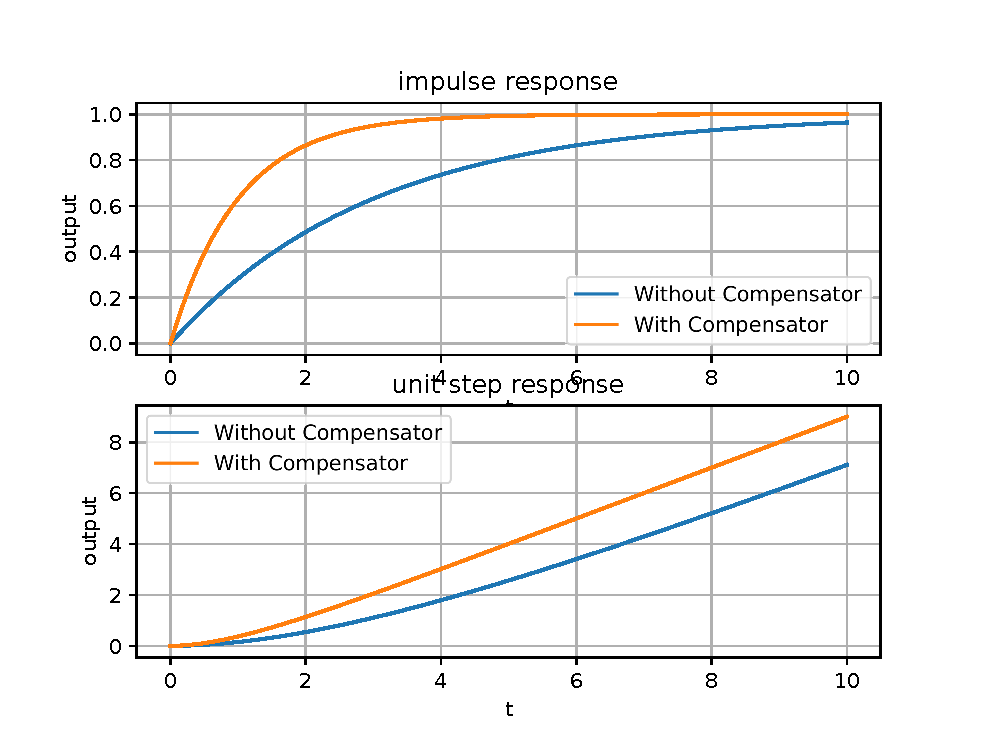
\includegraphics[width=1\linewidth, height=7cm ,inner]{./figs/ee18btech11027/settling_time.eps} 
\label{fig:subim1}
%\end{subfigure}
\end{figure}
Hence, from both examples we can see that settling time is reduced by using a lead compensator.\\

\textbf{Theoritically -}
Since lead compensator adds + phase for any value of frequency, the bode plot for phase vs frequency is above the one which is without lead compensator.\\

phase margin \phi_m = 180 + \phi_{gain = 0}\\
as\ lead\ compensator\ adds\ additional\ phase\\
at\ all\ frequencies, \\
$\phi_{gain = 0}$ \ gets increased, and hence\ phase\ margin.\\

Relation between phase margin and damping ratio.\\

\zeta = 0.01 $\times$ \phi_m\\

From this we get that damping factor also increases with phase margin.\\

\implies damping\ is\ increased \\

\implies settling\ time\ decreased\\

Deriving a relation between phase margin and damping ratio.
Consider a second order system,
\begin{align}
G(s) = \frac{\omega_n^2}{s^2+2\zeta\omega_ns+\omega_n^2} 
\end{align}
using value of $\phi_m$ to solve for $\zeta$.\\

set 20 $\log{|G(s)|}$ = -3dB to solve for \omega_n\\

using this equations we get,\\
\begin{align}
\phi_m = \tan^{-1}{\frac{2\zeta}{\sqrt{\sqrt{1+4\zeta^4} - 2\zeta^2}}}
\end{align}\\
a handy relation is - \zeta = 0.01\phi_m\\

\begin{figure}[h]
 \textbf{phase margin vs damping ratio}
\begin{subfigure}{\textwidth}
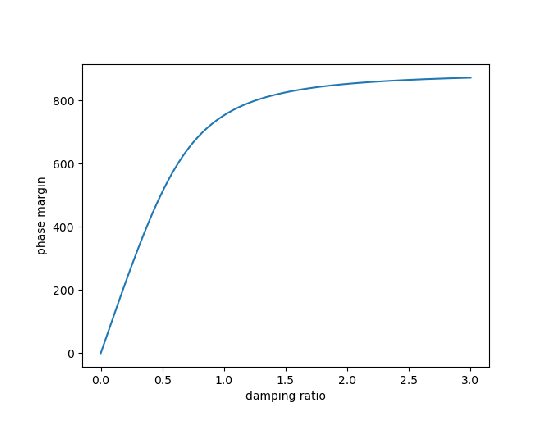
\includegraphics[width=1\linewidth, height=7cm ,inner]{./figs/ee18btech11027/realtion.eps} 
\label{fig:subim1}
\end{subfigure}
\end{figure}
\end{enumerate}

Hence,the settling time is reduced by using a lead compensator.\\
Similarly if we use a lag compensator the settling time increases as the phase margin decreases.